% !TEX encoding = UTF-8
% !TEX TS-program = pdflatex
% !TEX root = ../Lahmer_Abdelilah_tesi.tex
% !TEX spellcheck = it-IT

%**************************************************************

\chapter{L'azienda}

%**************************************************************
\section{Profilo aziendale}
L'azienda presso la quale ho svolto il mio stage è Sopra Steria Group S.p.A, una delle imprese che propone una delle offerte più complete di servizi \textit{end to end} presenti oggi sul mercato.\\

\begin{figure}[H]
	\centering
   	
\includegraphics[width=0.6\textwidth]{immagini/logo_azienda}
   	\caption{Logo di Sopra Steria Group S.p.A. - Fonte: \url{https://goo.gl/vbAJ6D}}
\end{figure}

Sopra Steria è infatti tra i leader europei in ambito di trasformazione digitale, propone una delle più complete offerte di servizi di \textit{Consulting}, \textit{Systems Integration}, \textit{Software Development} e \textit{Business Process Services} presenti oggi sul mercato.
Essa spazia su diversi mercati come \textit{Fashion}, \textit{Insurance}, \textit{Banking}, \textit{Retail}, \textit{Energy}, Aeronautica, Industria e Servizi, Sanità, Settore pubblico, Difesa e Trasporti.\\

Sopra Steria Group è partner di riferimento delle principali aziende ed organizzazioni pubbliche e private proponendo progetti di trasformazione di successo per affrontare al meglio le sfide di business più critiche e complesse, combinando un'alta qualità dei servizi erogati, valore aggiunto e innovazione.\\

L'azienda conta più di 40.000 collaboratori in più di 20 paesi, vanta inoltre un fatturato di 3,7 miliardi di euro nel 2016. Nello specifico opera sul territorio italiano con più di 800 risorse distribuite nelle sue sedi di Ariano Irpino (AV), Assago (MI), Asti, Collecchio (PR), Padova e Roma, fatturando circa 56,9 milioni nel 2016.\\

\begin{figure}[htbp]
\centering
\begin{minipage}[c]{.40\textwidth}
\centering\setlength{\captionmargin}{0pt}%
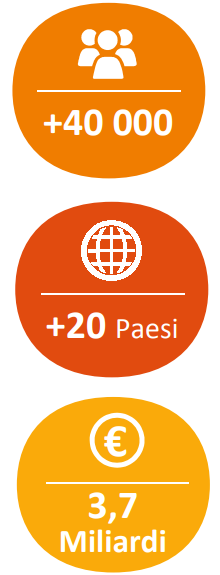
\includegraphics[width=0.6\textwidth]{immagini/dipendenti_paesi_fatturato_mondo}
\caption{Dati generali Sopra Steria nel Mondo}
\end{minipage}%
\hspace{10mm}%
\begin{minipage}[c]{.40\textwidth}
\centering\setlength{\captionmargin}{0pt}%
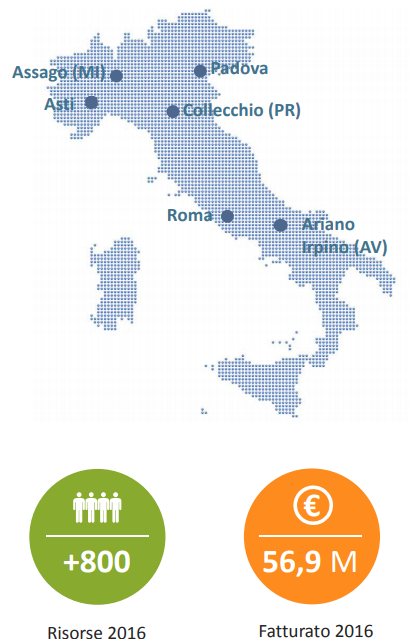
\includegraphics[width=1.2\textwidth]{immagini/mappa_italia_fatturato}
\caption{Dati generali Sopra Steria in Italia}
\end{minipage}
\caption{Informazioni generali Sopra Steria Group S.p.A. - Fonte: documento interno aziendale}
\end{figure}


Il gruppo è il risultato di una fusione avvenuta nel 2014 ad opera di due aziende, Sopra Group SA e Groupe Steria SCA, comunemente chiamate Sopra e Steria, fondate rispettivamente nel 1968 e 1969. Ad oggi l'azienda si presenta internamente ben strutturata in \textit{Business Unit}\footnote{Da questo punto per indicare il termine \textit{Business Unit} userò a volte anche il corrispettivo termine in italiano, ovvero Divisione.} relative agli ambiti di sviluppo e adotta una politica di \textit{recruiting} che mira alla competenza dei dipendenti da cui deriva la qualità dei prodotti, punto di forza dell'azienda.\\

Io sono stato inserito nella divisione "793 - Servizi Finanziari e Assicurazioni" della sede di Padova, nata negli ultimi anni a partire da pochi dipendenti e che ora conta circa 20 dipendenti solo per la sede in cui ho avuto il piacere di collaborare, senza contare i colleghi situati nelle sedi di Collecchio e Roma che cooperano anch'essi agli stessi progetti per la stessa divisione.\\
In particolare il mio ruolo è stato quello del sviluppatore \textit{host} e Analista Funzionale. \\
	Sono stato affiancato quindi da vari colleghi a seconda della tecnologia o conoscenza che dovevo apprendere. Più nello specifico sono stato affiancato dal mio collega Stefano Gori e dal mio tutor aziendale Marco Valentino, uno dei principali sviluppatori \textit{host} e manager di prossimità di questa sede, per l'apprendimento dei linguaggi COBOL\glossario\ e JCL\glossario. Sono stato invece affiancato dalle mie colleghe Chiara Maccotta e Francesca Constantini per l'apprendimento dei concetti teorici in ambito economico.\\ % essenziali per poter aver un quadro generale di quale sia lo scopo pratico del prodotto su cui si lavora e di una base teorica che permetta di raggionare sui risultati ottenuti dopo implementazioni e rispettivi risultati ottenuti.
	
	In quella che è la struttura aziendale i due ruoli per cui sono stato formato, ovvero quello di sviluppatore \textit{host} e Analista Funzionale, sono due mansioni a stretto contatto, in certi casi ricopribili ibridamente anche dallo stesso soggetto. \\ Più nel dettaglio l'incarico di Analista Funzionale consiste nel raccogliere i requisiti del cliente, tramite incontri ed interviste, ed il relazionarsi con esso al fine di capire ciò di cui ha bisogno. Con la redazione dei vari documenti di analisi questa figura deve essere in grado di portare all'interno del gruppo di sviluppo tutte le informazioni necessarie e sufficienti al successo della soluzione che verrà adottata. Nel contesto aziendale e di progetto in cui sono stato inserito io, avendo a che fare con istituti di credito, chi ricopre questo ruolo generalmente ha un \textit{background} più economico che tecnico, o in alternativa ha una pluriennale esperienza come sviluppatore tale per cui riesce comunque a tradurre le nozioni finanziarie in nozioni tecniche indirizzate agli sviluppatori. \\ Per quanto riguarda la mansione di sviluppatore \textit{host} invece consiste nel tradurre ciò che elaborano gli analisti in soluzione software mediante applicazioni in linguaggio COBOL. Generalmente chi ricopre questo ruolo ha un \textit{background} più tecnico che economico.\footnote{Da questo punto le descrizioni delle caratteristiche aziendali faranno riferimento alla \textit{Business Unit} in cui sono stato inserito, ovvero la "793 - Servizi Finanziari e Assicurazioni". Questo dato che ognuna di esse opera secondo logiche, ambiti e tecnologie differenti.}


%**************************************************************
\section{Prodotti e servizi offerti}
	
	\subsection{Prodotti}
	
	Nei mercati francesi, dove l'azienda è radicata, è attiva la vendita di prodotti bancari già pronti e configurabili in poco tempo presso i clienti. In Italia la situazione è differente e per i principali clienti, nell'ambito finanziario, raramente si vendono pacchetti di prodotti finiti ma si adotta una politica di personalizzazione secondo le esigenze del cliente. I prodotti principali offerti dalla \textit{Business Unit} in cui sono stato formato sono quindi riassumibili in:
		
	\begin{itemize}
		\item Applicazioni \textit{web} per la gestione di finanziamenti bancari, assieme alla relativa evoluzione e manutenzione;
		\item Programmi \textit{host} di gestione dati, gestione dei calcoli assieme alla consistenza e persistenza dei dati che vengono elaborati;
		\item Applicazioni \textit{web} utilizzabili dalla clientela degli istituti di credito.
	\end{itemize}
	
	\subsection{Servizi}
	
	Il sistema di gestione per la qualità dei servizi offerti ai clienti di Sopra Steria Group è certificato ISO 9001:2015 ed è annualmente sottoposto a verifiche da parte di un ente accreditato di terza parte.\\

	\begin{figure}[H]
	\centering
   	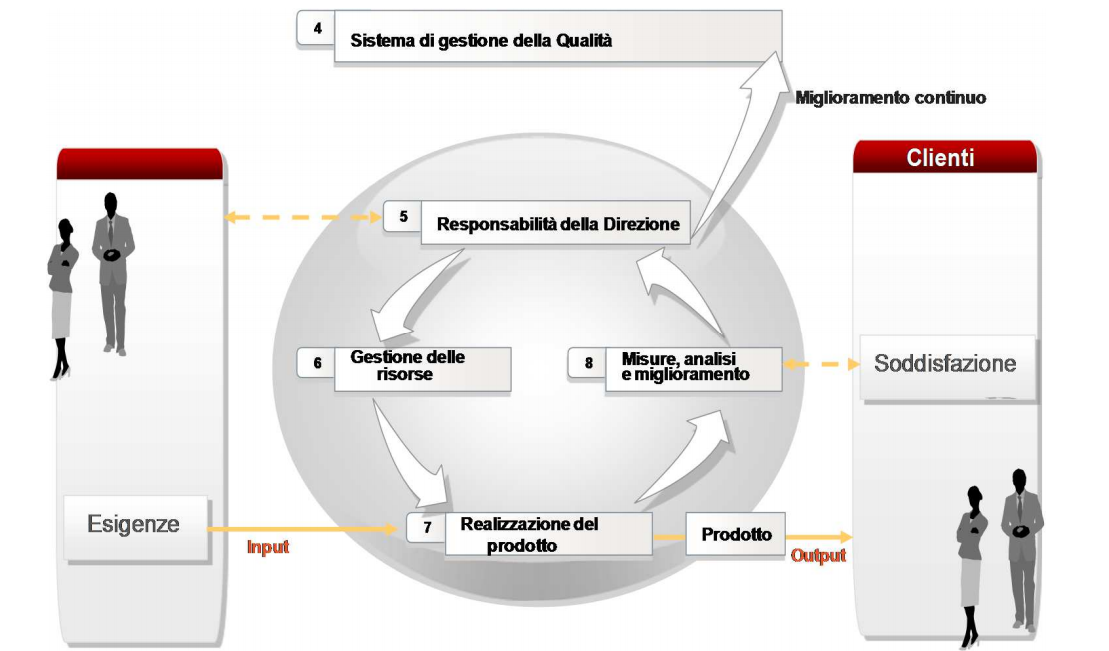
\includegraphics[width=0.85\textwidth]{immagini/ISO9001}
   	\caption{Politica della qualità di Sopra Steria Group S.p.A. - Fonte: documento interno aziendale}
	\end{figure}
	
	
	I principali servizi erogati dalla divisione per i clienti sono:
	
	\begin{itemize}
		\item Consulenza in ambito informatico per l'ampliamento ed il soddisfacimento della clientela da parte dei commerciali;
		\item Analisi delle necessità del cliente e dei conseguenti requisiti software;
		\item Progettazione e realizzazione di nuove applicazioni o nuove funzionalità di applicativi già in uso;
		\item Verifica e collaudo del software prodotto con finale rilascio nei sistemi del cliente;
		%\item Manutenzione dei contenuti proposti al cliente in un'ottica a lungo termine;
		\item Formazione del personale utilizzatore del prodotto, in particolare in seguito al rilascio di nuove funzionalità;
		\item Assistenza degli istituti bancari in caso si verifichi qualsiasi tipo di problema inerente al prodotto fornito.
	\end{itemize}	 

%**************************************************************
%\newpage
\section{Processi aziendali}

	\subsection{Organizzazione interna}
	
	L'organizzazione interna di Sopra Steria Group S.p.A. è un'organizzazione prettamente gerarchica	 che si sviluppa non solo a livello di direzione e sedi italiane ma a livello mondiale. Infatti le grandi dimensioni dell'azienda implicano questa forte strutturazione interna, assieme ad un'attenta gestione delle attività di coordinamento. Durante lo stage ho avuto modo di osservare molti degli aspetti di questo complesso sistema, anche inizialmente con la richiesta di tirocinio, che ho visto risalire lungo la gerarchia piramidale sino al consenso del direttore di \textit{Business Unit} e poi ritornare a livelli più bassi, dove una delle assistenti delle risorse umane mi ha notificato l'accettazione della richiesta.\\
	
	Una delle prime cose che si imparano di quest'azienda è la sua propensione alla cura dei rapporti con il cliente, poiché vengono offerte numerose sessioni	di consulenza. La filosofia è quella di collaborare per aiutarli a trasformare i loro sistemi informativi e, grazie all'esperienza del settore, offrire valore aggiunto mediante le soluzioni. Per raggiungere tale scopo il gruppo ha stretto delle \textit{partnership} strategiche con Microsoft, IBM, Oracle e HP. La missione principale del gruppo è di industrializzare e ottimizzare le proprie operazioni per migliorare la competitività e le  \textit{performance} in un'ottica a lungo termine.\\
	
	Un altro aspetto a cui l'azienda tiene in particolar modo è la gestione delle risorse umane. Sostenere lo sviluppo dell'evoluzione di queste ultime è considerata una priorità per il successo aziendale e per mantenere un alto livello di soddisfazione e di motivazione dei dipendenti. Per questo Sopra Steria si impegna a conoscere i profili e le competenze di ciascun collaboratore, al fine di poter offrire agli stessi prospettive di crescita e percorsi di carriera in grado di soddisfare sia le loro aspettative che il mercato. A tale scopo l'azienda organizza annualmente il cosiddetto PAP, acronimo che sta per \textit{Plan Annuel de Progression} ovvero Piano di Progressione Annuale, che serve appunto a favorire la crescita delle risorse; durante questo evento infatti i dipendenti vengono esaminati seguendo uno schema ben preciso e se le conoscenze dimostrate sono tali da potersi assumere responsabilità più grandi, questa possibilità di crescita viene valutata. Il colloquio PAP permette inoltre al collaboratore e al suo manager di prossimità di fare un bilancio del periodo appena trascorso e di fissare gli obiettivi e il piano di crescita per l'anno a venire. Durante questo evento si ha anche la possibilità di evidenziare l'esigenza di formazione e di accompagnamento per una gestione coerente della carriera. Il piano di crescita così elaborato rappresenta un impegno reciproco assunto dal collaboratore e dal suo superiore.% Fase importante della vita professionale, il colloquio PAP è un momento privilegiato di dialogo con l'azienda attraverso delle figure di riferimento, quali i Manager di Prossimità.\\
	
	%La crescente complessità dei progetti, la molteplicità degli interlocutori e le esigenze di alto livello dei clienti sono tali da comportare rischi considerevoli per l'azienda. L'intervento della direzione legale si rende pertanto necessario per difendere al meglio gli interessi del gruppo, tutelando i rapporti contrattuali con i clienti e le fasi di contenzioso, i rapporti con le software house, le parti terze, i partner e i fornitori e le acquisizioni o cessioni di attività.
	
	Per quanto riguarda il governo e la gestione del gruppo, i diversi livelli di poteri decisionali, sia a livello funzionale che produttivo, sono distribuiti nella gerarchia operativa oltre che nella direzione. Alla base di ciò, un'organizzazione complessa si ramifica nelle varie nazioni in cui l'azienda si estende, delegando l'amministrazione di questi filoni e di altri reparti di supporto a manager selezionati. A livello più basso si collocano le \textit{Business Unit}, ovvero le varie divisioni aziendali adibite all'erogazione di determinate tipologie di prodotti e servizi identificate anche in base al mercato di riferimento. Anche queste ultime risultano distribuite nel territorio, in ogni filiale infatti possono coesistere più reparti.\\
	
	\begin{figure}[H]
	\centering
	   	\includegraphics[width=0.8\textwidth]{immagini/Mercati_Principali}
	   	\caption{Suddivisione aree di mercato dell'azienda - Fonte dati: documento interno aziendale}
	\end{figure}
	
	Nella divisione in cui sono stato collocato vi sono diverse figure che si occupano dei vari processi di produzione. In ordine gerarchico è presente un direttore di \textit{Business Unit} per l'amministrazione delle risorse della divisione, i \textit{Project Manager} per la gestione dei progetti e dei loro costi, gli Analisti Commerciali che si occupano delle relazioni con i clienti, i team di Analisti e Consulenti che si occupano dei requisiti del cliente e i team di sviluppo software, suddivisi in sviluppatori \textit{web} e sviluppatori \textit{host}.\\

	%\subsection{Modello Incrementale}
	\subsection{Ciclo di sviluppo}
	
	Il ciclo di sviluppo software adottato da Sopra Steria nella divisione "793 - Servizi Finanziari e Assicurazioni" dove sono stato inserito è un'implementazione del modello incrementale, questa scelta è dovuta al fatto che l'azienda tratta per la maggior parte dei casi progetti di grandi dimensioni, il più delle volte progetti già avviati, che richiedono aggiunte sulla base delle funzionalità essenziali già sviluppate. Questo modello si caratterizza inoltre per la capacità di adattamento a molteplici tipologie di problemi.\\
	
	I punti di forza del procedimento incrementale sono i seguenti:
	\begin{itemize}
		\item L'integrazione delle parti del sistema è distribuita nel tempo e non collassata nelle fasi finali;
		\item La suddivisione in sottoinsiemi della realizzazione del problema comporta una migliore conoscenza di esso e una sua gestione più semplificata;
		\item Ogni incremento porta valore aggiunto, con lo sviluppo di nuove funzionalità e il soddisfacimento di alcuni requisiti;
		\item Ad ogni incremento si guadagnano esperienza e affidabilità, riducendo i rischi di fallimento;
		\item Le funzionalità essenziali sono sviluppate nei primi incrementi e attraversano più fasi di verifica, diventano quindi più stabili con ciascuna iterazione; questo sistema di \textit{rilasci multipli e successivi} permette anche al proponente di seguire in maniera attiva la prosecuzione del progetto avendo un'idea concreta del prodotto in corso di sviluppo.
	\end{itemize}
	
	 Questo modello si caratterizza inoltre per la capacità di adattamento a molteplici tipologie di problemi, in aggiunta si presta bene alle necessità dell'azienda perché i clienti richiedono che vengano effettuati lavori di manutenzione e amplificazione definibili in attività distinte, assimilabili facilmente tramite un ciclo di sviluppo ad incrementi. In figura vengono rappresentate le fasi del modello.\\
	
	\begin{figure}[H]
		\centering
	   	%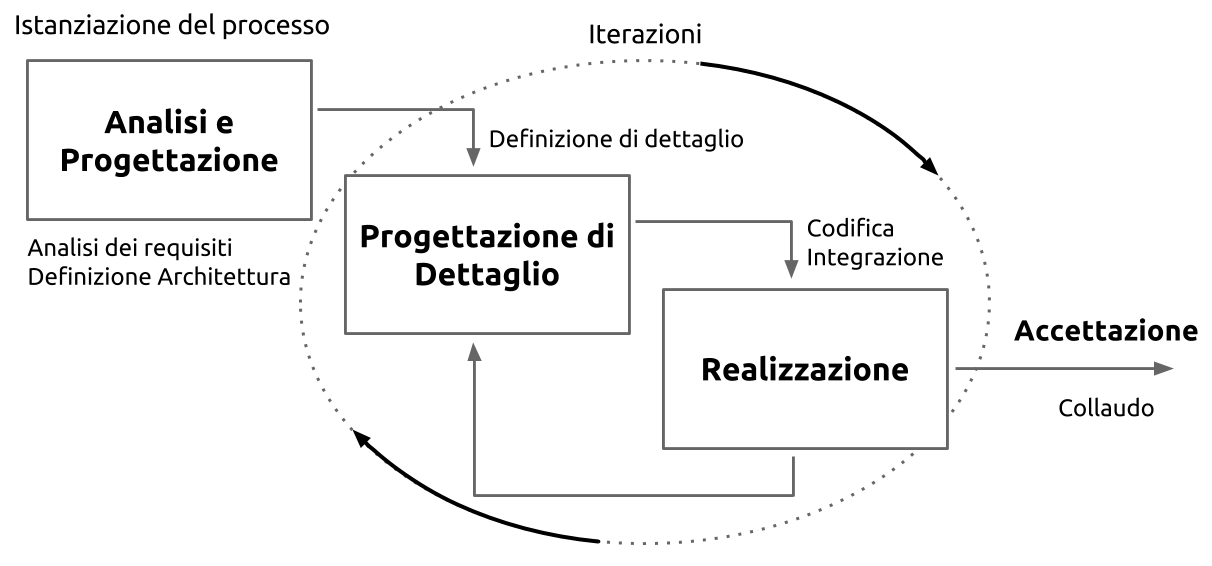
\includegraphics[width=1\textwidth]{immagini/modello_incrementale}
	   	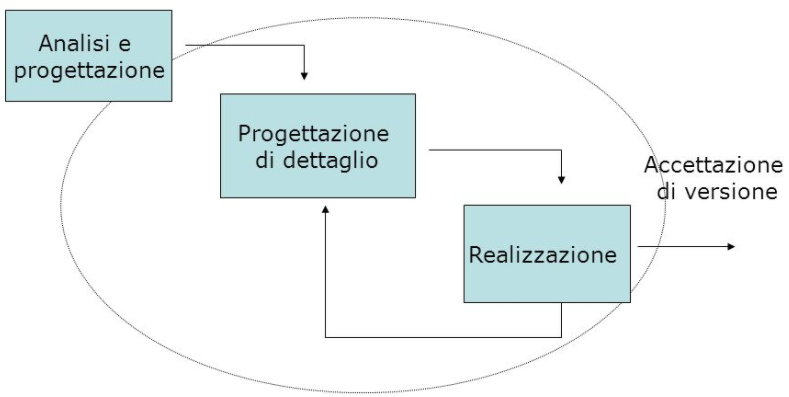
\includegraphics[width=1\textwidth]{immagini/ModelloIncrementale}
	   	%\caption{Modello di sviluppo incrementale}
	   	\caption{Modello di sviluppo incrementale - Fonte: \url{https://goo.gl/ZcNU8P}}
	\end{figure}
	%\newpage
	
	Il modello incrementale è un ciclo di sviluppo definito dallo standard ISO 12207 che combina la logica del modello a cascata, dove ogni fase è rigidamente sequenziale, e la filosofia iterativa della prototipazione.\\
	
	È prevista una prima fase di analisi dei requisiti fondamentali e di progettazione architetturale intesa a stabilire le fondamenta del software. Tale fase è essenziale per definire i successivi incrementi e non si ripete.\\
	
	Le fasi successive di realizzazione incrementale vera e propria, possono ripetersi più volte e mirano ad attività di progettazione di dettaglio, codifica e test, in cui vengono trattati prima i requisiti obbligatori, poi quelli facoltativi passando per quelli desiderabili. Le implementazioni subiscono i trattamenti di integrazione e collaudo, successivamente avviene un eventuale rilascio.\\

	È prevista la prototipazione delle nuove funzionalità che si vanno ad implementare per la validazione complessiva del sistema, reiterando 
	alle fasi di progettazione e realizzazione in caso di errori o problematiche. In questo modo è possibile di volta in volta acquisire maggiore competenza riguardo al problema, riducendo i rischi successivi e le tempistiche globali di produzione software.
	
	%\subsection{}
	\paragraph{Il modello incrementale in Sopra Steria}
\leavevmode	\newline \newline
	Ogni ciclo di incremento inizia con la raccolta e l'analisi dei requisiti presso il cliente, che espone le sue necessità tramite riunioni oppure mediante opportuna documentazione.\\
	
	Questo procedimento di raccolta dei requisiti e stesura dei documenti di analisi avviene generalmente dalle figure di Analisti Funzionali. Questi si occupano di raggruppare i requisiti in macro attività, calcolare le tempistiche necessarie per il loro completamento e stilare i documenti di \textit{Analisi Funzionale}. Dopo la stesura di tale documento, questo viene esposto al proponente al fine di approvazione. In caso il cliente ritenga che questo documento non sia adatto alle richieste o che ci siano delle mancanze viene notificato e gli analisti provvedono alle dovute correzioni. Questo procedimento di correzione della documentazione e attesa di approvazione può ripetersi sino alla giunta dell'accettazione da parte del proponente.\\
	
	Una volta approvato il documento entra in gioco la figura del \textit{Responsabile Commerciale} che presenta ai clienti un preventivo per l'implementazione delle funzionalità richieste.\\ %Pure questo preventivo passa all'approvazione del proponente e solo
	
	Una volta ottenuta l'accettazione dell'offerta commerciale si da il via alla stesura del documento di \textit{Analisi Tecnica} in cui si evince la progettazione di dettaglio. Tale documentazione risulta necessaria ai vari team di sviluppo per la comprensione e l'applicazione delle implementazioni richieste, ma non indispensabile per alcuni di essi.\\
		
	Gli analisti rimangono a disposizione degli sviluppatori anche nelle fasi successive per eventuali chiarimenti e specificazioni, in modo da non rallentare o interrompere le fasi successive. I documenti vengono inviati ai team competenti a cui sono state attribuite le macro attività e da quel momento inizia la realizzazione. Tali gruppi di lavoro possono risultare distribuiti nelle varie sedi del territorio italiano, perciò sono previste molte comunicazioni telefoniche o tramite posta elettronica e occasionali trasferte, al fine di allineare le procedure di sviluppo o rendere noto quando è possibile procedere con determinate modifiche. \\
	
	L'evoluzione degli incrementi software attraversa ambienti distinti. Esistono in particolare i seguenti ambienti:
	\begin{itemize}
		\item \textbf{Sviluppo}: ambiente di programmazione locale, qui avviene l'implementazione delle modifiche software;
		\item \textbf{Integrazione}: in questo ambiente vengono raccolte le implementazioni delle attività e si verifica che non generino conflitti, mediante test di non regressione\footnote{Con test di non regressione si intendono i test tali per cui si prova che, in eseguito alla modifica di una parte P del sistema S, la modifica di P non abbia introdotto errori né in P né alle altre parti di S che hanno relazione con P.}, garantendo la stabilità del sistema;
		\item \textbf{Collaudo}: ambiente di validazione delle funzionalità complessive del software, utilizzato anche per dimostrare al cliente la loro consistenza;
		\item \textbf{Produzione}: questo ambiente varia per ogni cliente o applicazione sviluppata e rappresenta lo stato finale del prodotto in cui viene effettivamente utilizzato dal cliente.
	\end{itemize}	
	
	È responsabilità del programmatore che prende in carico lo sviluppo delle funzionalità dichiarare il loro completamento, almeno a livello di prototipo, per rilasciarlo in integrazione. Determinati team si occupano poi di testare l'applicazione nelle sue nuove funzioni, accertando il soddisfacimento dei requisiti ed eventualmente contattando gli analisti per eventuali modifiche progettuali. In caso di problematiche le modifiche vengono respinte in ambito di sviluppo altrimenti vengono approvate per il collaudo. In collaudo è possibile utilizzare le funzioni sviluppate da altri team e validare il lavoro svolto per presentarlo poi al cliente, rilasciando in produzione la nuova versione del software.
	
	%\subsection{Strumenti a supporto di processi e servizi}
	\subsection{Tecnologie e strumenti a supporto di processi e servizi}

	Nel corso dello stage sono stati utilizzati numerosi strumenti di supporto per facilitare lo svolgimento delle diverse attività, dai tool di gestione delle basi di dati all'analisi del codice scritto passando per la gestione di progetto. Al fine di fornire ai suoi collaboratori tutti gli strumenti utili a rendere al meglio, Sopra Steria Group fornisce un portale da cui chiunque può scaricare o richiedere uno strumento, debitamente giustificato; tutto ciò affinché persista un alto livello di soddisfacimento e di motivazione dei dipendenti, che come abbiamo detto parlando di organizzazione interna è un punto sul quale l'azienda conta molto. Il portale porta il nome di \textbf{IT CORP} che abbinato al portale principale aziendale denominato Face2Face e il servizio sottostante di IT Request permettono di ottenere in qualsiasi momento applicativi o qualsivoglia strumento necessario nell'ambiente lavorativo.

	\begin{figure}[H]
		\centering
	   	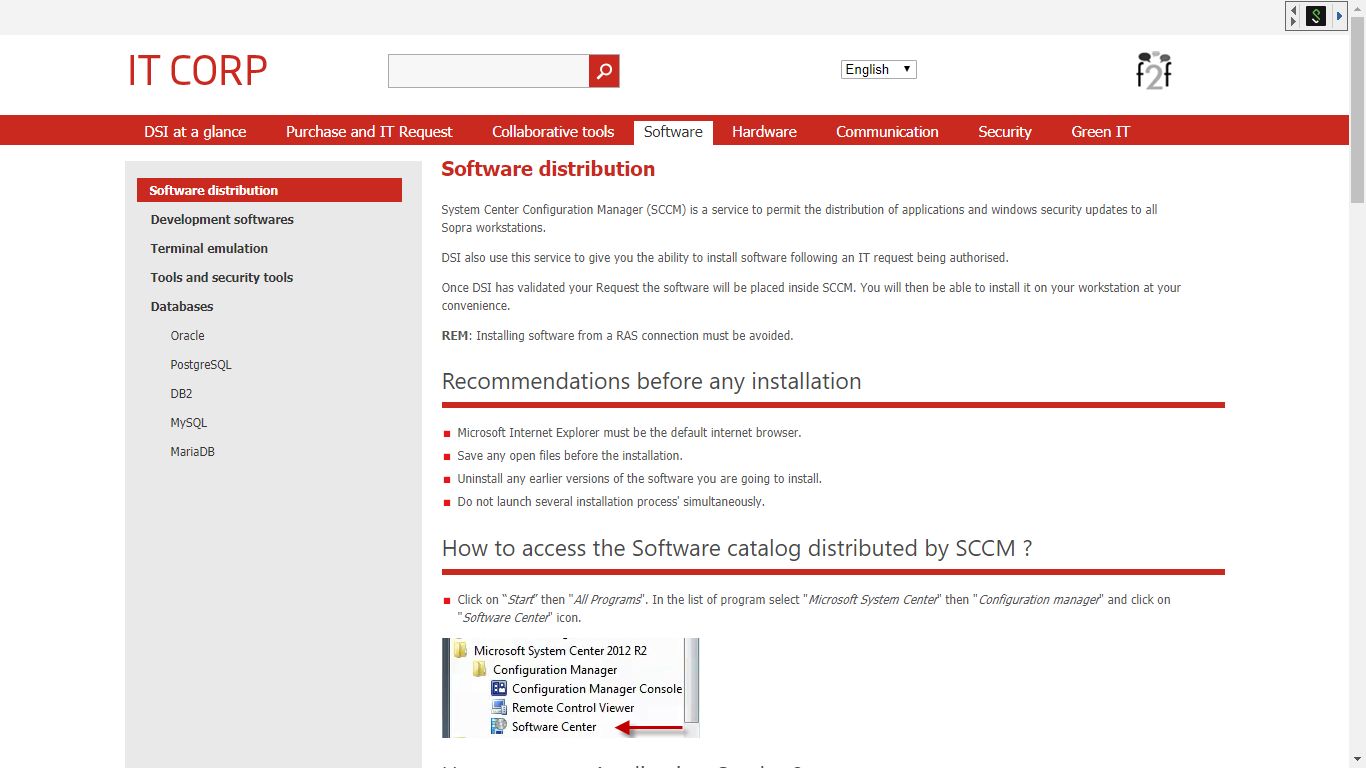
\includegraphics[width=1\textwidth]{immagini/ITCorp}
	   	\caption{La pagina iniziale di IT CORP - Fonte: Portale interno dell'azienda}
	\end{figure}
	
	La scelta degli strumenti è basata sulla pluriennale esperienza del team, che ha scelto gli strumenti con cura, dopo un attento studio delle funzionalità offerte di ognuno, attenendosi a vari fattori tra cui il supporto presente online e facilità di utilizzo, in modo da assicurare un'alta qualità dei processi. Di seguito saranno descritte le principali funzionalità e caratteristiche dei vari strumenti.\\

	Parlando di ambiente lavorativo della divisione "793 - Servizi Finanziari e Assicurazioni" e strumenti a supporto di processi e servizi all'interno di essa non si può non distinguere inizialmente e prima di tutto le due macrocategorie di ruoli che un dipendente di questa \textit{Business Unit} può assumere, ovvero la categoria degli sviluppatori \textit{Web} e quella degli sviluppatori \textit{Host}. Ognuna di queste due famiglie opera secondo politiche diverse, utilizzando processi e strumenti ben distinti. Di seguito quindi saranno descritte le principali funzionalità e caratteristiche dei vari strumenti specificando se si tratta di uno strumento a supporto della prima categoria di sviluppatori o della seconda.
	
	\subsubsection{Linguaggi}
	
	I linguaggi di programmazione utilizzati dagli sviluppatori facenti parte della divisione dove sono stato inserito sono molteplici, essendo che quest'ultima lavora su vari progetti in distinte sedi italiane. Discuterò quindi solo delle tecnologie utilizzate all'interno del progetto su cui lavora il team di cui ho fatto parte durante lo stage.
		
	\subsubsection{Linguaggi lato Host}
	Durante il periodo di stage gran parte delle attività di formazione si sono concentrate sui linguaggi da usare lato \textit{host}, ovvero i linguaggi COBOL e JCL.\\
	
	Il linguaggio \textbf{COBOL} è un linguaggio che risale agli ultimi anni '50, il suo nome è un acronimo che sta per COmmon Business-Oriented Language. Come si capisce dal nome esteso questo linguaggio è prettamente orientato al business, la traduzione del nome esteso infatti è "\textit{linguaggio comune orientato alle applicazioni commerciali}", e questo è infatti l'uso che se ne fa generalmente, ovvero programmi di gestione di sistemi bancari e assicurativi.\\

	I principali vantaggi di cui godeva il COBOL rispetto ai linguaggi che gli facevano concorrenza al tempo sono stati: 
	\begin{itemize}
		\item L'aritmetica con il punto decimale fisso, fattore molto utile nei programmi con funzioni di contabilità, che troviamo molto nel dominio bancario e in quello delle assicurazioni;
		\item Una maggiore velocità di input/output;
		\item Una sintassi con un'ottima leggibilità, conferita dal fatto che è simile a quella della lingua inglese;
		\item La capacità di gestione di enormi volumi di elaborazione con facilità.
	\end{itemize}		

	Con lo sviluppo e il perfezionarsi di questo linguaggio versione per versione, si è giunti a quella del 2002 con la quale il COBOL subiva una svolta significativa, ovvero il supporto della programmazione orientata agli oggetti.\\
	 
	Il linguaggio \textbf{JCL}, invece, è un linguaggio che anch'esso risale alla seconda metà del XX secolo ed è un acronimo che sta per Job Control Language. Il JCL è un linguaggio di \textit{scripting} generalmente utilizzato nei sistemi operativi IBM per eseguire (in gergo lanciare) una procedura batch\glossario\ su un sistema in genere mainframe. Nello specifico, lo scopo del JCL è quello di dire quali programmi eseguire, usando quali file di input e quali generare in output. L'uso che se ne fa nel contesto aziendale in cui sono stato inserito è principalmente quello di programmare e regolare l'esecuzione di programmi che generalmente vengono eseguiti periodicamente.

	\subsubsection{Linguaggi lato Web}

	Dovendo sviluppare anche l'applicativo web gli sviluppatori web su questo
fronte hanno scelto di adottare la piattaforma Java per il web (\textbf{Java EE}) e ovviamente le tecnologie standard relative alla presentazione e al comportamento delle pagine, ovvero \textbf{HTML}, \textbf{CSS} e \textbf{JavaScript}.\\

\begin{figure}[htbp]
\centering
\begin{minipage}[c]{.40\textwidth}
\centering\setlength{\captionmargin}{0pt}%
\captionsetup{width=1.2\linewidth}

\includegraphics[width=0.7\textwidth]{immagini/JavaEE}
\caption{Logo Java EE - Fonte: \url{https://goo.gl/wckR1M}}
\end{minipage}%
\hspace{15mm}%
\begin{minipage}[c]{.40\textwidth}
\centering\setlength{\captionmargin}{0pt}%
\captionsetup{width=1.25\linewidth}

\includegraphics[width=1\textwidth]{immagini/HTML5_CSS_JavaScript}
\caption{Logo HTML5, CSS3 e \\JavaScript - Fonte:\\ \url{https://goo.gl/A72tDP}}
\end{minipage}
\caption{Tecnologie utilizzate dagli sviluppatori Web}
\end{figure}
		
	L'edizione di Java che utilizzano gli sviluppatori Web è Java Platform Enterprise Edition, comunemente chiamata Java EE, che è un'estensione di Java SE (Standard Edition) e rappresenta una piattaforma di sviluppo software molto usata per applicazioni d'impresa.\\
	
	La versione di HTML utilizzata invece è la HTML5, che è l'ultima \textit{release} di HTML, risponde alle esigenze moderne ed alle aspettative dei siti web. Una delle caratteristiche principali di questa ultima edizione è il concetto di markup semantico, ovvero la capacità di fornire informazioni sul contenuto che descrive un dato tag. Oltre a questa particolarità, un'altra qualità che spicca è la capacità di adattarsi perfettamente, ovvero ad avere il medesimo comportamento sia su desktop che su mobile. \\
	
	Per tutti questi aspetti HTML5 è diventando un nuovo standard per gli sviluppatori web, tant'è che è diventato \textit{W3C Recommendation} dall'ottobre 2014.\\

	Per quanto riguarda il comportamento delle pagine web invece si è optato per l'uso della versione CSS3 per la gestione della formattazione delle pagine e di JavaScript per le validazioni e controlli \textit{client-side}.
		
	\subsubsection{Database}
	Il salvataggio dei dati per le applicazioni in ambito bancario e assicurativo avviene generalmente tramite DBMS\glossario\ relazionali come DB2 di IBM, Microsoft SQL Server e MySQL di Oracle. Il team di sviluppo in base anche ai calcolatori a disposizione della banca, anch'essi della IBM, ha scelto di utilizzare il \textbf{DB2}, che è nato nel 1983 ma tutt'oggi è uno tra gli RDBMS\glossario\ più usati, specie in questo settore. In origine era nato come DBMS per i mainframe CICS\glossario\, poi si è diffuso su diversi tipi di server. Per questo banche e assicurazioni, enti che esistono da molto prima della nascita del DB2, inizialmente hanno adottato questa tecnologia mediante sistemi EIS\glossario\ implementati in linguaggio COBOL che tutt'oggi gli forniscono le funzionalità necessarie senza il bisogno di adottare tecnologie più moderne e sviluppate secondo le esigenze dei più recenti paradigmi di programmazione.\\
	
	L'amministrazione delle basi di dati avviene tramite uno strumento denominato \textbf{DBeaver}, che è un applicazione gratuita multipiattaforma per sviluppatori, programmatori, amministratori di dabases e analisti.%Supporta più tipologie di database come MySQL, PostgreSQL, Oracle, DB2, SQL Server, MS Access e molti altri.% Teradata, SQLite, Sybase, Firebird, MariaDB, Derby 

	\begin{figure}[H]
	\centering
	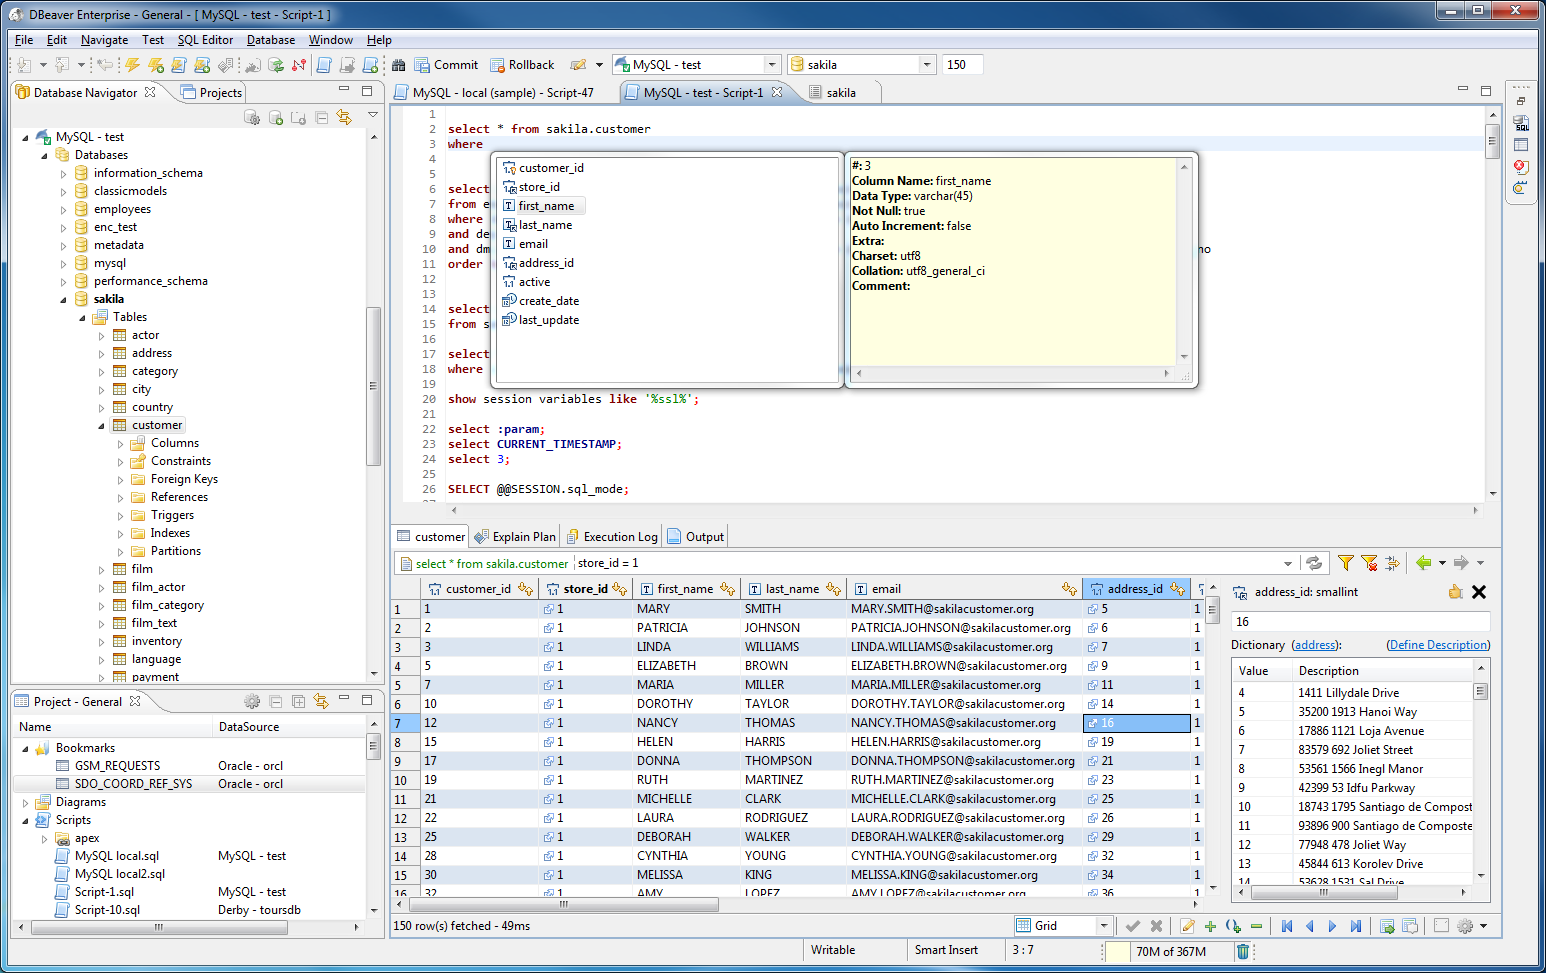
\includegraphics[width=0.85\textwidth]{immagini/DBeaver_ss}
	\caption{Schermata dello strumento di amministrazione dei databases DBeaver - Fonte: \url{https://github.com/serge-rider/dbeaver}}
	\end{figure}

	\subsubsection{Ambienti di sviluppo ed emulatori}
	\label{Ambienti di sviluppo ed emulatori}

	Anche parlando di ambienti di sviluppo è importante distinguere quelli usati lato sviluppatori \textit{web} e quelli usati lato sviluppatori \textit{host}.\\
		
	Il principale ambiente di sviluppo adottato per le applicazioni web è \textbf{Eclipse}. Esso racchiude la globalità delle caratteristiche necessarie ad uno sviluppatore in questo ambito. Rappresenta un'ottima soluzione e agevolazione per il processo di sviluppo, in quanto offre funzionalità di collegamento ai sistemi di versionamento, \textit{debugging} del codice \textit{runtime}, oltre alle molteplici caratteristiche offerte dai comuni editor di testo orientati allo sviluppo dei sorgenti software.\\
	
%	\begin{figure}[H]
%		\centering
%	   	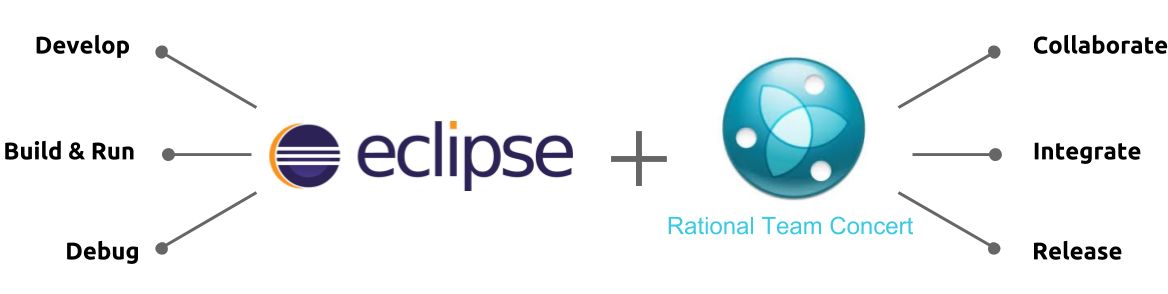
\includegraphics[width=0.7\textwidth]{immagini/ambienti_sviluppo}
%	   	\caption{I vantaggi dell'uso di Eclipse in collaborazione con RTC}
%	\end{figure}
	
	Altri programmi di supporto sono invece i diversi browser in cui bisogna testare il funzionamento delle pagine web tra cui Internet Explorer, Firefox e Chrome e gli editor di testo utili in situazioni dov'è richiesta più praticità come Notepad++.\\

	Il principale ambiente di sviluppo adottato lato \textit{host} invece è \textbf{ISPF}\glossario. Esso include vari tool e funzionalità per la gestione dell'intero processo di sviluppo dei programmi \textit{host}; dalla creazione dei programmi al versionamento degli stessi, dall'analisi statica del software in fase di compilazione alla gestione della base di dati tramite lo strumento QMF\glossario.

	\begin{figure}[H]
		\centering
	   	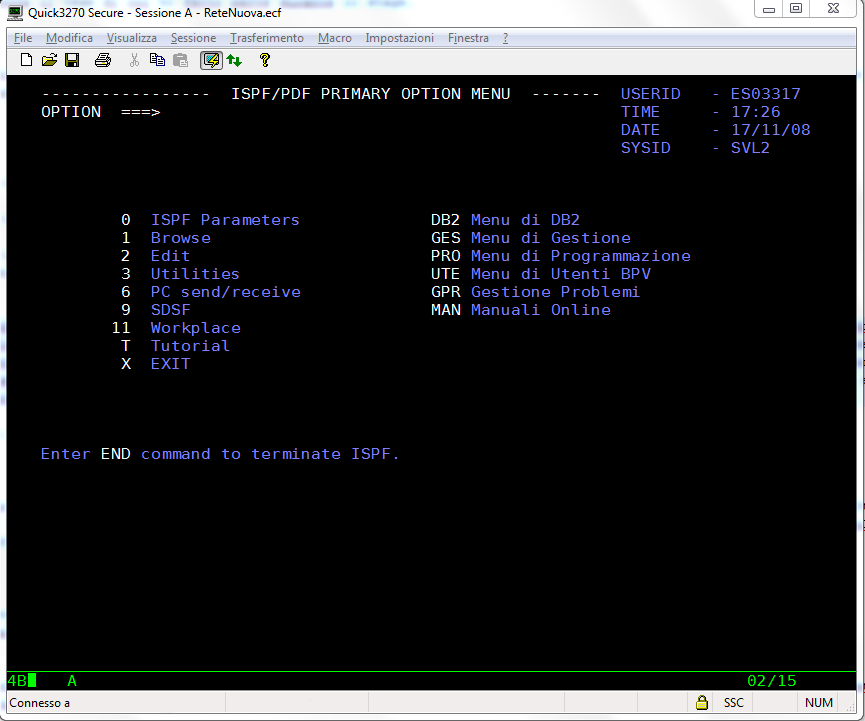
\includegraphics[width=0.80\textwidth]{immagini/ISPF}
	   	\caption{Schermata iniziale ambiente di sviluppo ISPF}
	\end{figure}

	Durante il periodo di stage ho avuto modo di imparare ad usare gran parte dei \textit{tool} che mette a disposizione ISPF, assistendo anche all'utilizzo di alcune funzionalità a cui sono abilitate solo un determinato tipo di utenze, ovvero le cosidette \textit{utenze di produzione}, che sono quelle con il totale accesso anche ai database e ai sistemi collocati dal cliente, e non solo a quelli di test su cui lavorano il resto degli sviluppatori.\\
	
	La struttura del menu di questo ambiente di sviluppo è indicativamente come illustrato nel seguente schema:
	
	\begin{figure}[H]
		\centering
		\captionsetup{width=0.70\linewidth}
	   	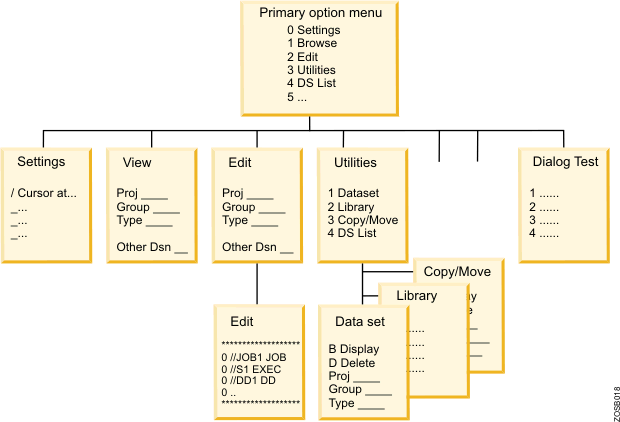
\includegraphics[width=0.80\textwidth]{immagini/ISPF_menu_structure}
	   	\caption{Struttura menu ambiente di sviluppo ISPF - Fonte: \url{https://goo.gl/GX6P9V}}
	\end{figure}

	Per utilizzare ISPF in azienda ho utilizzato l'emulatore \textbf{Quick3270 Secure} che è un potente ed affidabile emulatore di terminali IBM 3270 e IBM 5250. Utilizzabile su sistemi operativi Windows questo programma permette infatti di connettere il proprio computer ai sistemi IBM zSeries (S/390) e iSeries (AS/400).

	\subsubsection{Gestione di progetto}

	A supporto della gestione delle attività progettuali Sopra Steria mette a disposizione dei suoi dipendenti un portale comune che permette la gestione dei gruppi di lavoro. Oltre alle funzionalità di gestione di progetto questo portale permette anche l'organizzazione della comunità aziendale e favorisce il dialogo organizzato dipendente-azienda, seppur virtuale.\\
	
	Il portale aziendale, \textbf{Face2Face}, gestisce molteplici attività e problematiche. Tramite esso i dipendenti sono tenuti a riportare settimanalmente le proprie attività di lavoro e gli ambiti di progetto al fine di inviare i dati alla direzione, permettendole di coordinare le risorse a disposizione. Lo strumento consente inoltre di consultare le news aziendali e gli eventi organizzati.

	\begin{figure}[H]
		\centering
	   	\includegraphics[width=1\textwidth]{immagini/Face2Face}
	   	\caption{La Home Page di Face2Face - Fonte: portale interno dell'azienda}
	\end{figure}
		
	Face2Face è accessibile anche dall'esterno della rete aziendale tramite un portale online predisposto dall'azienda. In questo modo viene facilitato il lavoro in trasferta dei dipendenti.\\
	
	\subsubsection{Documentazione}
	
	Nell'arco della mia permanenza in azienda per lo stage ho avuto modo di vedere quella che è la documentazione che la prassi aziendale vuole che venga redatta. Per ogni attività risultante dall'analisi dei requisiti, infatti, vengono stilati due documenti: l'\textit{Analisi Funzionale} e l'\textit{Analisi Tecnica}. In fase di rilascio delle funzionalità richieste durante la fase di analisi vengono redatti invece i documenti di \textit{Collaudo} e quello di \textit{Rilascio}.\\
	
	Il primo documento, ovvero quello di Analisi Funzionale, affronta i requisiti ad alto livello, enunciando le principali funzionalità ed i cambiamenti rispetto alla versione attualmente in produzione dell'applicativo.\\
	
	\leavevmode	\newline

	Le sezioni principali di questo documento sono:
\begin{itemize}
	\item Matrice dei requisiti: enunciato discorsivo per introdurre il problema proposto;
	\item Descrizione funzionale: per spiegare il comportamento dell'applicativo lato web, presentando possibilmente anche un'anteprima delle pagine che verranno aggiunte;
	\item Casi oggetto di collaudo: qui vengono indicate le componenti che saranno analizzate in fase di  \textit{testing} per verificarne il corretto comportamento;
	\item Dettaglio tecnico: qui vengono enunciate le componenti software che saranno modificate o aggiunte, senza entrare nel dettaglio di come tali modifiche andranno apportate.
\end{itemize}

	Il secondo documento invece, ovvero quello di Analisi Tecnica, affronta nel dettaglio gli aspetti tecnici che vanno modificati o aggiunti trattando principalmente i programmi COBOL lato \textit{host}, dai quali poi anche i programmatori web possono individuare i parametri da utilizzare nelle richieste via rete per recuperare i dati e quindi allinearsi.\\
	
	Il documento di Analisi Tecnica, diversamente da quello di Analisi Funzionale non sempre viene steso visto che questo non ha obbligo di approvazione da parte del cliente e quindi, in particolari casi, gli sviluppatori con più esperienza sono in grado di progettare e sviluppare la parte tecnica in autonomia senza l'aiuto di quest'ultimo.\\
	
	Al termine dello sviluppo dei requisiti, ad avvenuta validazione, vengono inoltre redatti i documenti di Collaudo e di Rilascio, da consegnare al cliente per accertare i lavori eseguiti e il rilascio delle nuove funzionalità.\\
			
	Il software utilizzato per la produzione dei documenti è \textbf{Microsoft Word}, i cui formati sono standard sia per l'azienda che per i clienti.
	
	
	\subsubsection{Sistemi di versionamento}

	Come precedentemente accennato nella sezione riguardante gli ambienti di sviluppo [\ref{Ambienti di sviluppo ed emulatori}], lo strumento \textbf{ISPF} permette, in un certo qual modo, il versionamento dei programmi sorgenti lato \textit{host}. Questo infatti tiene traccia di ogni modifica apportata ai programmi e consente quindi di ripristinare una versione di un dato modulo utilizzando un progressivo numerico, identificativo di una certa versione del software, che si incrementa ogni qualvolta questo viene modificato e compilato.\\
	
	Per quanto riguarda il lato web, invece, nel progetto su cui lavora il team in cui sono stato inserito il sistema di versionamento del software utilizzato è \textbf{RTC} (Rational Team Concert, IBM), che è costruito su IBM Jazz, una piattaforma estensibile che aiuta i team ad integrare i task attraverso il ciclo di vita del software. RTC dispone di un'architettura client-server e permette ai team di sviluppo di tenere traccia del loro lavoro in modo intuitivo.
	
	\subsubsection{Sistemi operativi}
	
	Per le postazioni di sviluppo è previsto un sistema centralizzato di utenze a cui è attribuito un proprio ambiente di lavoro ed uno spazio assegnato a cui accedere da qualsiasi computer aziendale.\\
	
	Nelle macchine aziendali è consueto l'utilizzo di Microsoft Windows 7 come sistema operativo primario per ovviare a discrepanze nelle postazioni dei diversi dipendenti e per omogenizzare ulteriormente il processo di sviluppo. Questo comporta una buona soluzione per concentrarsi unicamente sul proprio lavoro e avere al contempo una garanzia nell'utilizzo quotidiano.
	
%**************************************************************

%\section{Clientela e trasformazione digitale}
\section{Clientela ed innovazione}

	\subsection{Clientela target}
	
	La clientela target della \textit{Business Unit} "793 - Servizi Finanziari e Assicurazioni" di Sopra Steria sono principalmente gruppi bancari e assicurativi. Essi solitamente necessitano una qualche forma di innovazione o evoluzione che gli garantisca continuità di produzione ma anche i corretti adeguamenti previsti dai cambiamenti legislativi.\\
	
	 Per permettere questo, gli analisti si incaricano di entrare in contatto con i responsabili ICT\glossario\ della società cliente, dai quali poi si ricavano le diverse richieste implementative;  che possono andare dalla variazione di qualche caratteristica alla creazione di funzionalità completamente nuove.\\

	%\subsection{Principali clienti e progetti}
	
	Visto il successo conquistato con il passare degli anni Sopra Steria Group si è sempre fatta strada tra i brand più importanti in vari settori, tra i quali i seguenti, classificati per aree di mercato.
	\begin{figure}[H]
	\centering
   	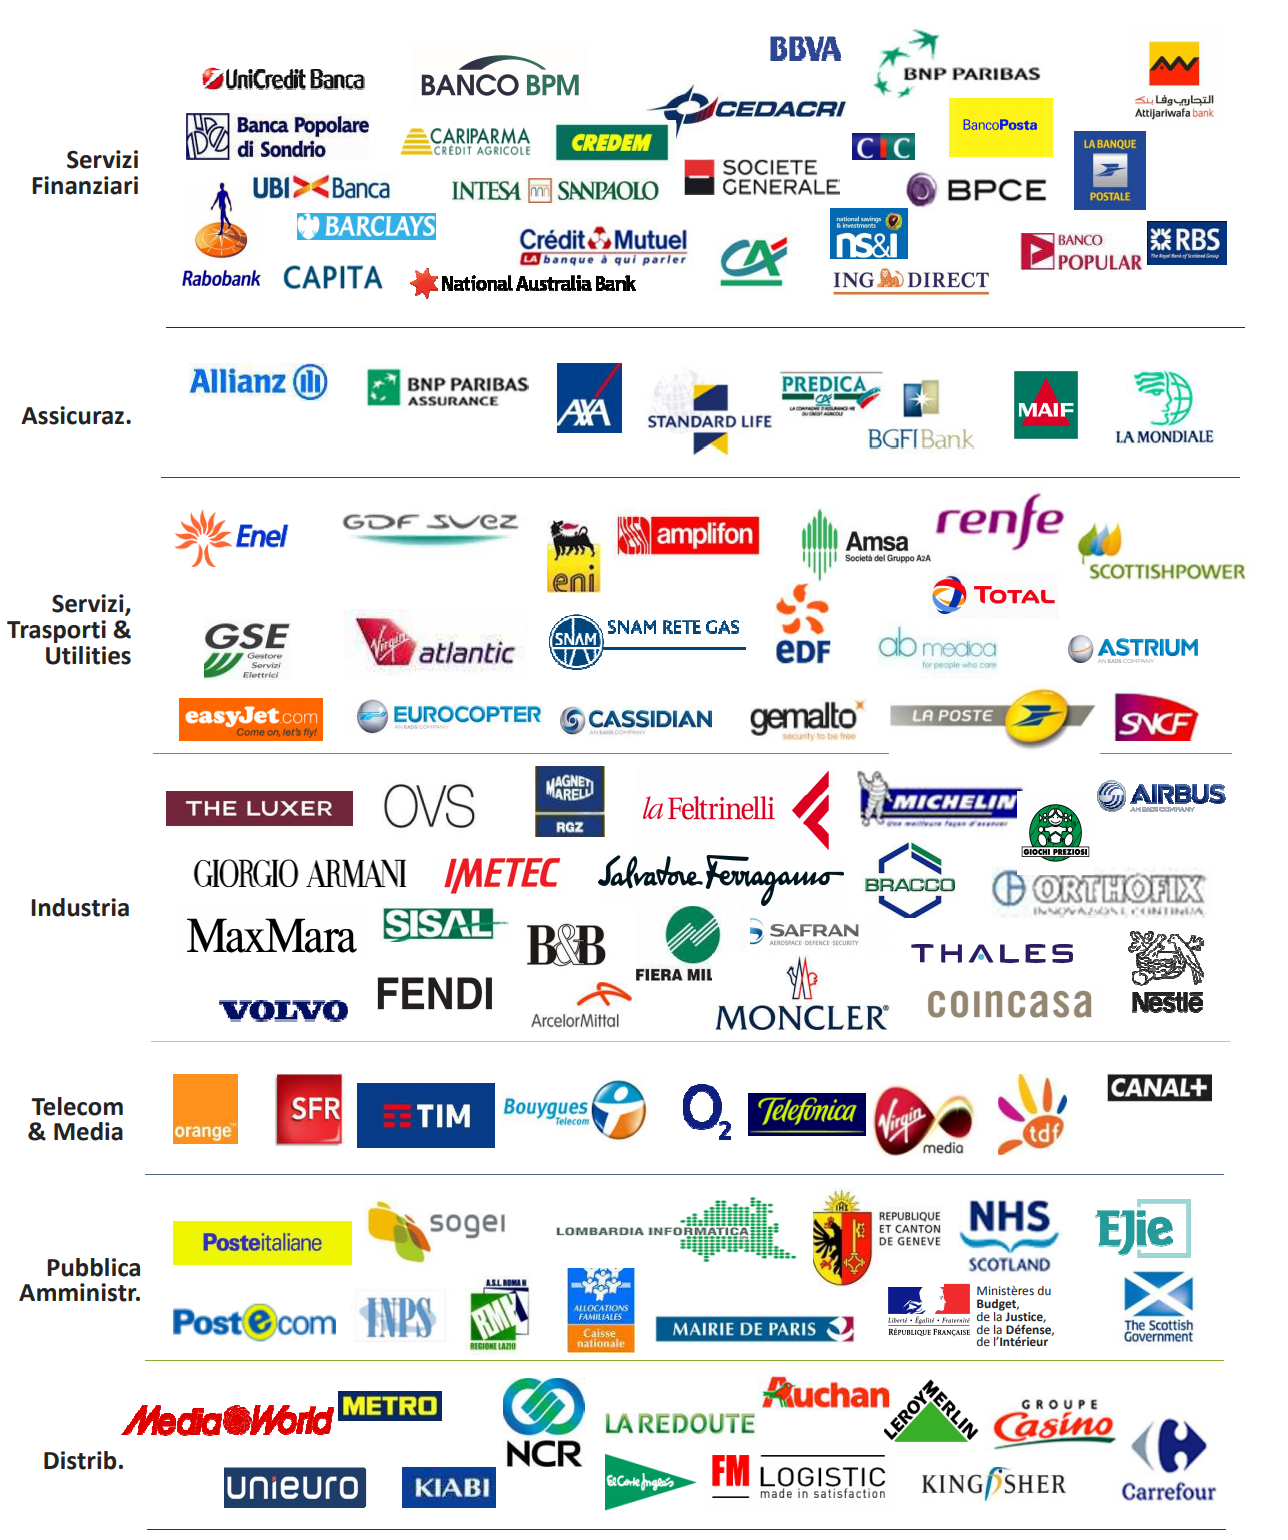
\includegraphics[width=0.7\textwidth]{immagini/principali_referenze}
   	\caption{Principali clienti di Sopra Steria Group S.p.A. - \\Fonte: documento interno aziendale}
	\end{figure}

	I progetti di maggior impatto, invece, per cui Sopra Steria è riuscita ad ottenere il privilegio di approvvigionamento e conseguente implementazione sono stati molteplici, tra questi citiamo i seguenti.
	\begin{figure}[H]
	\centering
   	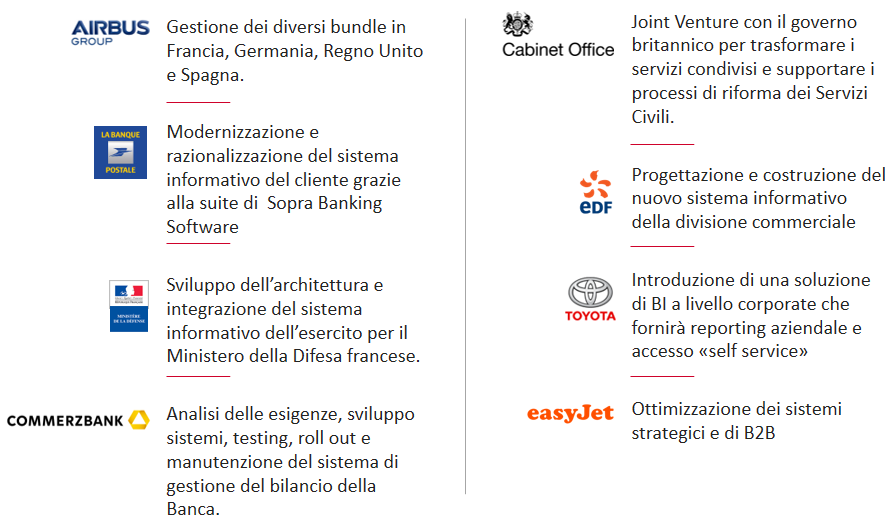
\includegraphics[width=0.76\textwidth]{immagini/Progetti_Importanti}
   	\caption{Principali progetti di Sopra Steria Group S.p.A. - \\Fonte: documento interno aziendale}
	\end{figure}

	
	\subsection{Innovazione}
	
	L'innovazione e le soluzioni software richieste dalle banche e assicurazione non sono mai stati termini accostabili. %, soprattutto negli ultimi anni.
	Se da un lato le tecnologie stanno subendo una rivoluzione importante dall'altro lato gli istituti di credito preferiscono avere sistemi funzionanti e garantiti anche se il mantenimento degli stessi richiede somme non da poco. Se da un lato si parla di migrazione sul  \textit{Cloud} dei sistemi informativi delle aziende all'avanguardia dal lato degli istituti di credito si parla al più di cambio di versione dei  \textit{Framework} utilizzati lato  \textit{front-end}\glossario.\\

	\begin{figure}[H]
	\centering
	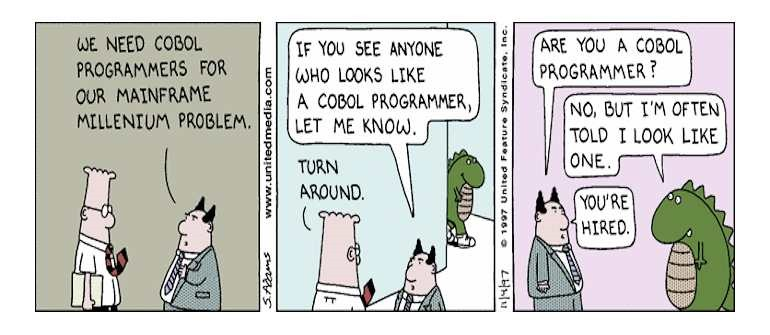
\includegraphics[width=0.85\textwidth]{immagini/VignettaCobol}
	\caption{Vignetta sull'uso del COBOL - Fonte: \url{https://goo.gl/dVnwEg}}
	\end{figure}
	
	L'innovazione in ambito bancario e assicurativo rappresenta infatti un'ostacolo non indifferente, questo tipo di enti sono da sempre legati a tecnologie primordiali come il linguaggio COBOL e la relativa implementazione in mainframe CICS.\\
	
	Per Sopra Steria, che fa della trasformazione digitale e innovazione un suo punto di forza, questo rappresenta una sfida, l'azienda infatti desidera mettersi in gioco offrendo le soluzioni adeguate, tenendo conto però delle priorità del cliente e delle sue possibilità. Queste caratteristiche sono molto ricercate dalle aziende che vogliono rinnovarsi, trasformando i loro processi e servizi nel mondo digitale, adeguandosi ai moderni canoni di utilizzo e facendosi avanti nei mercati, con la possibilità di offrire prodotti di maggiore qualità e raggiungere molti più clienti.\\
	
	Per quanto riguarda il progetto su cui lavora il team in cui sono stato inserito l'unico fattore di innovazione riguarda il lato  \textit{front-end} dell'applicazione, l'evoluzione infatti da questo lato si fa vedere mediante l'utilizzo di tecnologie moderne adatte alla presentazione dei contenuti	nel web, tecnologie che sono maggiormente soggette a spinte evolutive dovute alla modernizzazione degli standard.